\documentclass[a4paper]{article}
\usepackage{german}
\usepackage[utf8]{inputenc}

\pdfcompresslevel=0
\usepackage{pgfplots}

\usepackage{pgfplotstable}
\usepackage{booktabs}
\usepackage{array}
\usepackage{colortbl}

\begin{document}
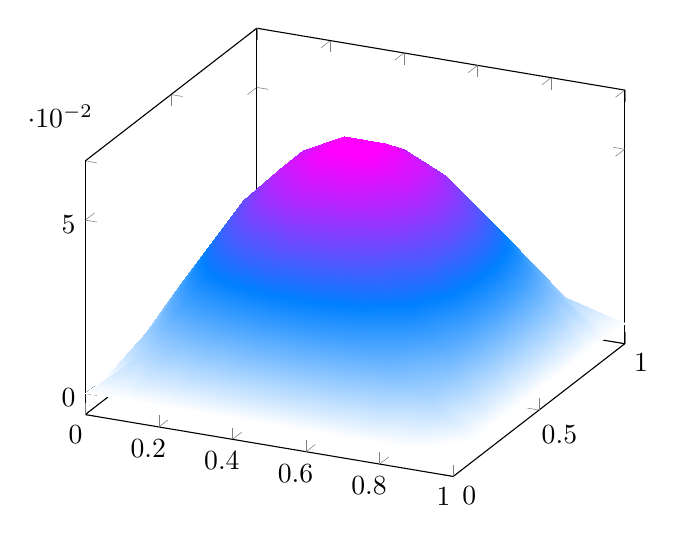
\begin{tikzpicture}
\begin{axis}[colormap/cool]
\addplot3[surf,samples=10,domain=0:1,
shader=interp]
{x*(1-x)*y*(1-y)};
\end{axis}
\end{tikzpicture}

\pgfdeclarehorizontalshading{myshadingA}
  {1cm}{rgb(0cm)=(1,0,0); color(2cm)=(green); color(4cm)=(blue)}
\pgfuseshading{myshadingA}

\end{document}

